\documentclass{article}
\usepackage{amsmath,amssymb,setspace,verbatim,graphicx,enumerate,enumitem}
\usepackage[top=1in,bottom=1in,left=1in,right=1in,head=0.5in,foot=0.5in]{geometry}
\usepackage{caption}
\usepackage{mathtools}
% \usepackage{subcaption}
% \usepackage{subfig}
% \usepackage{subfloat}
% \usepackage{tabularx}
\usepackage{mdframed}
\usepackage{amsthm}

\newtheorem*{theorem}{Theorem}

\newenvironment{Rcode}% environment name 
{%begin code
    \begin{mdframed}
    \#R code
    \begin{small}
}
{%end code
    \end{small}
    \end{mdframed}
}

\newenvironment{console}% environment name 
{%begin code
    \begin{mdframed}
    \#Console
    \begin{small}
}
{%end code
    \end{small}
    \end{mdframed}
}

\begin{document}
\title{STDA Homework 1}
\author{Seokjun Choi}
\date{April 10, 2020}
\maketitle

Note: \\
You can get full, run-able code files at my github page: Visit https://github.com/letsjdosth/SpaTempoDA \\
Because I provide the full code file separately, in this report,
I will show key-code block only instead of bringing the full, verbose code.

\section{Problem 1}
\textbf{
Suppose we want to simulate a random vector $Y \sim N(\mu, \Sigma)$.
If $\Sigma$ (Matern) is symmetric and positive definite, it can be represented using the
Cholesky decomposition $\Sigma = LL'$, where $L$ is a lower triangular matrix.
Consider the following algorithm for simulating Y:
\begin{itemize}
    \item Calculate the matrix $L$.
    \item Sample $Z \sim N(0,I)$, where $I$ is the $n \times n$ identity matrix.
    \item Let $Y=\mu+LZ$
\end{itemize}
}
\subsection{Problem 1-(a)}
\textbf{
Show that $Y$ generated in this way has the correct distribution.
You may use the fact that a linear function of a multivariate normal random variable is
again multivariate normal; just show the mean and variance are correct.
}

From the elementary observation from mathematical statistics, we have
for $a,b \in \mathcal{R}$ and for a random variable $X$,
\[E[aX+b] = aE[X]+b\]
\[Var[aX+b]=a^2 Var[X]\]
And its multivariate version is, for proper $A\in\mathcal{R}^{n\times n}$, $b\in\mathcal{R}^n$,
and for a random vector $X$,
\[E[Ax+b]=AE[X]+b\]
\[Var[AX+b]=AVar[X]A'\]
Then, using this observation and the fact at this problem, we can get
\[Y \sim N(\mu + 0, LIL')\]
Since $LL'=\Sigma$ by our setting, we get \(Y \sim N(\mu, \Sigma)\), so we can confirm that the algorithm is valid.



\subsection{Problem 1-(b)}
\textbf{
Write a function or a few lines of code in R to implement this method
for arguments mu and Sigma. You may use the built-in function chol for the Cholesky decomposition and rnorm to generate Z.
}

Here is implementation. 
Also you may see the 'HW1sol\_problem.R' file.

\begin{Rcode}
    \begin{verbatim}
rnorm_chol_algorithm = function(mu, Sigma) {
    # mu is vector
    # Sigma should be symmetric, positive definite matrix
    dimension = dim(Sigma)
    vecZ = rnorm(dimension, 0, 1)
    chol_upperL = chol(Sigma)
    return(mu + t(chol_upperL) %*% vecZ)    
}
    \end{verbatim}
\end{Rcode}



\subsection{Problem 1-(c)}
\textbf{
For a mean and covariance function of your choosing, use your code from (b) and
make a few plots illustrating realizations of a Gaussian process on [0;1], but changing the different parameters in the model.
These differences will be easier to see if you keep the same Z sample but just change mu and Sigma.
}

For convenience, I use fields\$Matern function to calculate covariance matrix from parameters of Matern.
Here are 3 test cases. (In full code, there are one more case for ordinary(not Matern) GP.)
\begin{itemize}
    \item $\nu = 0.1$ (in code, test 3)
    \item $\nu = 0.5$ (in code, test 2)
    \item $\nu = 1$ (in code, test 4)
\end{itemize}
Note that $\nu = 0.5$ case is the exponential covariance.



\begin{figure}[hh]
    \centering
    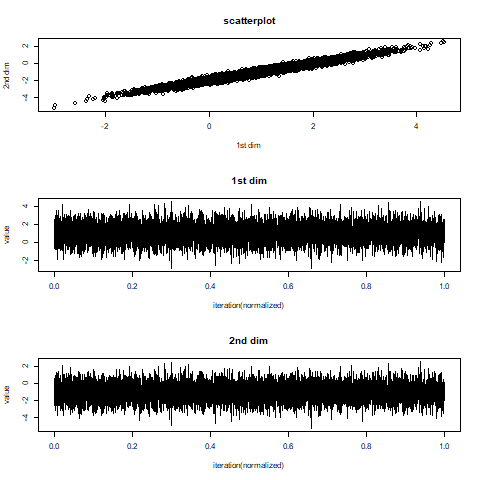
\includegraphics[height=8cm]{prob1_test3_scatter.png}
    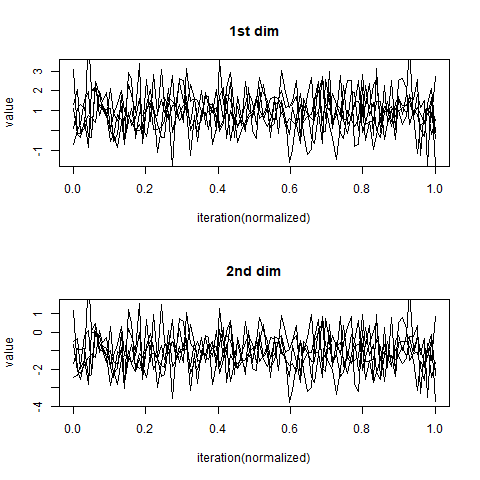
\includegraphics[height=8cm]{prob1_test3_traceplot.png}
    \caption{$\nu=0.1$}
\end{figure}




\section{Problem 2}
The file CAtemps.RData contains two R objects of class SpatialPointsDataFrame, called CAtemp and CAgrid.
CAtemp contains a average temperatures from 1961-1990 at 200 locations (latitude and longitude) in California in degrees Fahrenheit, along with their elevation in meters.
CAgrid contains elevations in meters over a grid of locations.
I've given you some code to get started with this data in HW1.R

Consider the following model for the temperature data.
\[Y_i = \mu(s_i;\beta) + e(s_i; \sigma^2, \rho, \tau)\]
where \(\mu(s_i;\beta)=\beta_0+\beta_1 Longitude(s) + \beta_2 Latitude(s)
+\beta_3 Elevation(s)\) and \(e(s_i;\sigma^2,\rho,\tau)\) is a zero mean stationary Gaussian process with
exponential covariance function.

Another way of writing this is as
\[Y_i = \mu(s_i;\beta) + Z(s_i; \sigma^2, \rho) + \epsilon_i\]
where now $Z$ is mean zero Gaussian process like $e$ but without the nugget term,
and the $\epsilon$ are iid $N(0,\tau^2)$, independent of Z.
This is important because we want to predict \(\mu(s_i;\beta)+Z(s_i;\sigma^2,\rho)\) without the measurement error.



\subsection{Problem 2-(a)}
\textbf{
Using the CAtemp data, form a preliminary estimate of $\beta$ using ordinary least squares 
and make a color plot of the residuals.
Include your estimates and plot.
}


\subsection{Problem 2-(b)}
\textbf{
Estimate the variogram non-parametrically and then fit the exponential variogram to it using weighted least squares.
Make and include a plot of the nonparametric and parametric variogram functions.
Also store your parameter estimates and report them.
}


\subsection{Problem 2-(c)}
\textbf{
We will now form the GLS estimate of $\beta$ by hand, rather than using the gls function.
\begin{itemize}
    \item Use the rdist function in fields to create a matrix of distance (in miles) between pairs of locations in CAtemp.
    \item Create the covariance matrix, plugging in your estimates from the fitted variogram. (Hint: Sum tow matrix, one without a nugget and one using the diag function to create the matrix $\tau^2 I$)
    \item Invert the covariance matrix and store it for later reference.
    \item Create the X matrix (Hint: Use cbind.)
    \item Put all the pieces together to form $\hat{\beta}_{GLS}$.
\end{itemize}
}


\subsection{Problem 2-(d)}
\textbf{
Calculate and plot the EBLUP of $\mu+Z$ at the location in CAgrid,
plugging in your estimates from (b) and (c).
Calculate and plot the (estimated) standard error of $Z$ at each prediction location
}


Since $Z \sim N(0, C)$, by definition of functional distribution in weak sense,
\(\langle Z, x\rangle \sim N(\langle 0,x \rangle, \langle C(x),x\rangle)\) for all $x\in \mathcal{H}=\mathcal{L}^2([0,1])$.
So, with eigenfunctions $\{v_i\}$, we get multivariate normal distribution for
\[\{\langle Z, v_i\rangle\}_{i=1,2,...,m} \sim Normal_m(
\begin{bmatrix}
    \langle 0,v_1 \rangle \\
    \langle 0,v_2 \rangle \\
    ... \\
    \langle 0,v_m \rangle
\end{bmatrix}
,
\begin{bmatrix}
    \langle C(v_1),v_1 \rangle & \langle C(v_1),v_2 \rangle & ... & \langle C(v_1),v_m \rangle \\
    \langle C(v_2),v_1 \rangle & \langle C(v_2),v_2 \rangle & ... & \langle C(v_2),v_m \rangle \\
    ... \\
    \langle C(v_m),v_1 \rangle & \langle C(v_m),v_2 \rangle & ... & \langle C(v_m),v_m \rangle \\
\end{bmatrix}
)\]
For simplicity, denote above expression's covariance matrix as $\Sigma_m$. Then we simply write above as
\[\{\langle Z, v_i\rangle\}_{i=1,2,...,m} \sim Normal_m(0,\Sigma_m)\]
Since the pdf of multivariate normal is well known, I write it without additional explanation.
If denote the vector \([\langle Z, v_i\rangle]_i, i=1,2,...,m\) as $z_m$, then
\[
    f_m(z_m) = \frac{1}{(\sqrt{2\pi})^m det(\Sigma_m)}exp{(-\frac{1}{2}(z_m-0)^T\Sigma_m^{-1}(z_m-0))}
\]

Likewise, since $X:=\mu+Z$,
\[\{\langle X, v_i\rangle\}_{i=1,2,...,m} \sim Normal_m(
\begin{bmatrix}
    \langle \mu,v_1 \rangle \\
    \langle \mu,v_2 \rangle \\
    ... \\
    \langle \mu,v_m \rangle
\end{bmatrix}
,
\begin{bmatrix}
    \langle C(v_1),v_1 \rangle & \langle C(v_1),v_2 \rangle & ... & \langle C(v_1),v_m \rangle \\
    \langle C(v_2),v_1 \rangle & \langle C(v_2),v_2 \rangle & ... & \langle C(v_2),v_m \rangle \\
    ... \\
    \langle C(v_m),v_1 \rangle & \langle C(v_m),v_2 \rangle & ... & \langle C(v_m),v_m \rangle \\
\end{bmatrix}
)\]
with denoting the mean vector as $\mu_m$ covariance matrix as $\Sigma_m$. Then we simply write above as
\[\{\langle X, v_i\rangle\}_{i=1,2,...,m} \sim Normal_m(\mu_m,\Sigma_m)\]
and pdf is, where \(x_m=[\langle X, v_i\rangle]_i, i=1,2,...,m\),
\[
    f_m(x_m) = \frac{1}{(\sqrt{2\pi})^m det(\Sigma_m)}exp{(-\frac{1}{2}(x_m-\mu_m)^T\Sigma_m^{-1}(x_m-\mu_m))}
\]


\end{document}